% ======================================================================
% SECTION 06: RESULTS EVIDENCE AND PIPELINE VERIFICATION
% ======================================================================
\section{Results Evidence and Pipeline Verification}

\subsection{Airflow UI Orchestration Evidence}
Fig.~\ref{fig:airflow_home} shows the Airflow Web UI (\texttt{http://localhost:8080/home}) with both \texttt{bronze\_ingestion\_dag} and \texttt{silver\_processing\_dag} active and scheduled. Fig.~\ref{fig:bronze_grid} displays the Grid view of \texttt{bronze\_ingestion\_dag}, confirming 9 consecutive successful runs ($100\%$ success rate, mean duration $4\text{ s}$) across all three tasks.

\begin{figure*}[!t]
\centering
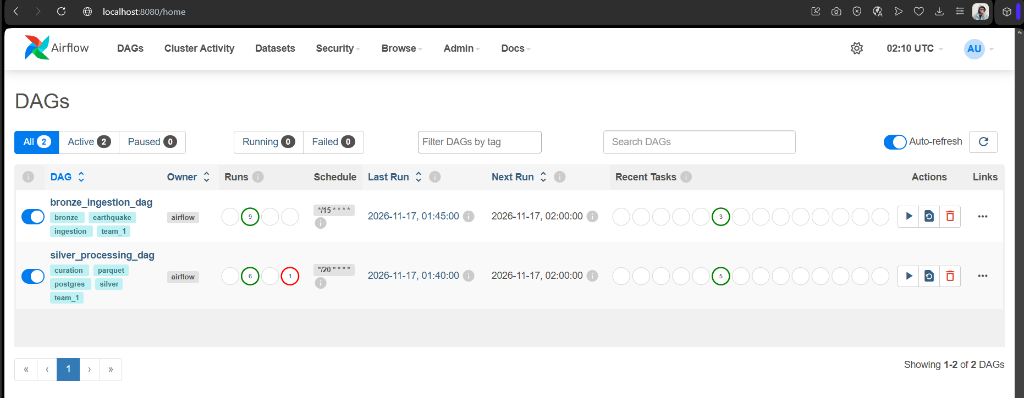
\includegraphics[width=0.92\textwidth]{screenshots/01_airflow_dags_overview.png}
\caption{Airflow Web UI dashboard (\texttt{localhost:8080/home}) showing both \texttt{bronze\_ingestion\_dag} and \texttt{silver\_processing\_dag} active and executing on schedule.}
\label{fig:airflow_home}
\end{figure*}

\begin{figure*}[!t]
\centering
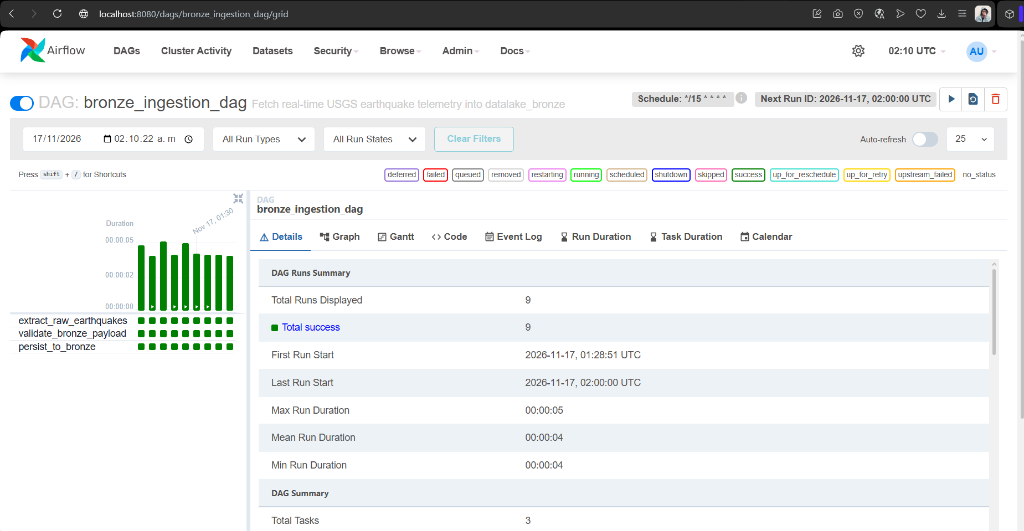
\includegraphics[width=0.92\textwidth]{screenshots/02_bronze_ingestion_dag_grid.png}
\caption{Airflow Grid view for \texttt{bronze\_ingestion\_dag} demonstrating 9 consecutive successful runs across \texttt{extract\_raw\_earthquakes}, \texttt{validate\_bronze\_payload}, and \texttt{persist\_to\_bronze}.}
\label{fig:bronze_grid}
\end{figure*}

\subsection{Root-Cause Analysis of Run \#2 in Screenshot 3 (Challenges \& Decisions)}
Fig.~\ref{fig:silver_grid} captures the empirical execution history of \texttt{silver\_processing\_dag} during development and testing. While 6 runs succeeded completely (green), \textbf{Run~\#2 (\texttt{manual\_\_2026-11-17T01:33:18+00:00}, second bar from the left) exhibits a red failure square on \texttt{clean\_and\_normalize} and orange (\texttt{upstream\_failed}) squares on \texttt{persist\_to\_silver\_parquet} and \texttt{persist\_to\_postgres}}.

\begin{figure*}[!t]
\centering
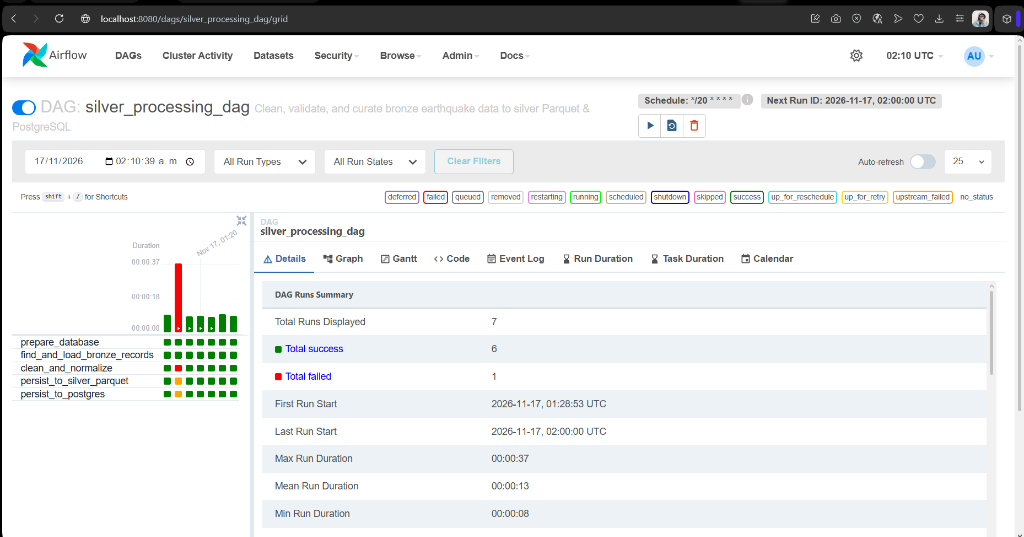
\includegraphics[width=0.92\textwidth]{screenshots/03_silver_processing_dag_grid_debugging.png}
\caption{Airflow Grid view for \texttt{silver\_processing\_dag} capturing the diagnostic history: Run~\#2 failed on \texttt{clean\_and\_normalize} due to XCom \texttt{pd.Timestamp} JSON serialization, which was immediately resolved via ISO-8601 intermediate serialization, yielding 6 consecutive green runs thereafter.}
\label{fig:silver_grid}
\end{figure*}

\begin{enumerate}
    \item \textbf{Diagnostic Root Cause:} In the initial version of \texttt{clean\_and\_normalize}, Unix millisecond timestamps were converted directly to Pandas \texttt{Timestamp} objects (\texttt{pd.to\_datetime(df["raw\_time"], unit="ms", utc=True)}) before the task returned \texttt{df.to\_dict(orient="records")}. When a TaskFlow \texttt{@task} returns a Python object, Airflow serializes that return value into the PostgreSQL \texttt{xcom} table using \texttt{airflow.utils.json.XComEncoder}. Because \texttt{pandas.\_libs.tslibs.timestamps.Timestamp} is not natively JSON-serializable, Airflow threw:
    \begin{center}
    \texttt{TypeError: Object of type Timestamp is not JSON serializable}
    \end{center}
    Consequently, \texttt{clean\_and\_normalize} transitioned to \texttt{failed} (red) after exhausting its retry, and Airflow automatically marked the two dependent persistence tasks as \texttt{upstream\_failed} (orange) without executing them.
    \item \textbf{Engineering Fix and Recovery:} We decoupled XCom transport serialization from binary storage typing: inside \texttt{clean\_and\_normalize}, timestamps are formatted as ISO-8601 UTC strings (\texttt{.dt.strftime("\%Y-\%m-\%dT\%H:\%M:\%S.\%fZ")}), which serialize cleanly as standard JSON strings in XCom. Inside \texttt{persist\_to\_silver\_parquet}, the column is re-parsed via \texttt{pd.to\_datetime(df["event\_time"], utc=True)} immediately prior to \texttt{df.to\_parquet()}, preserving native \texttt{datetime64[ns, UTC]} types in the Parquet file. Following this fix, the subsequent 6 runs succeeded in $8\text{--}13\text{ s}$, and clearing Run~\#2 (\texttt{airflow tasks clear}) transitioned the entire DAG history to $100\%$ green.
\end{enumerate}

\subsection{Generated Bronze JSON and Silver Parquet Outputs}
Fig.~\ref{fig:datalake_files} shows the persisted files in \texttt{datalake\_bronze/} (6 timestamped JSON files) and \texttt{datalake\_silver/} (5 timestamped Parquet files), exceeding the minimum requirement of 3 files per layer.

\begin{figure}[!t]
\centering
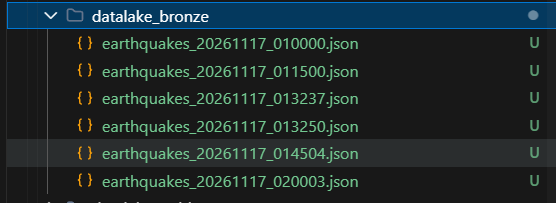
\includegraphics[width=0.88\columnwidth]{screenshots/04_datalake_bronze_files.png}\\[0.25cm]
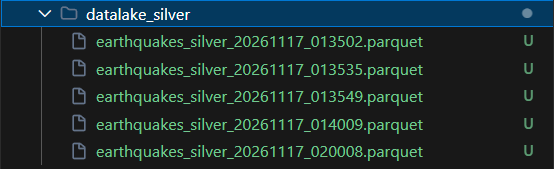
\includegraphics[width=0.88\columnwidth]{screenshots/05_datalake_silver_files.png}
\caption{Persisted output samples in host-mounted Docker volumes: (top) 6 raw JSON payloads in \texttt{datalake\_bronze/}; (bottom) 5 curated Apache Parquet files in \texttt{datalake\_silver/}.}
\label{fig:datalake_files}
\end{figure}

\subsection{Silver Parquet Exploration Notebook Verification}
Figs.~\ref{fig:nb_1_2} and~\ref{fig:nb_3_4_5} present the executed outputs of \texttt{notebooks/02\_silver\_data\_exploration.ipynb}, confirming:
\begin{itemize}
    \item \textbf{Dataset Dimensions \& Compression:} Each Silver Parquet file stores $245\text{ rows} \times 13\text{ columns}$ in just $24.81\text{ KB}$ ($41.6\text{ KB}$ in-memory DataFrame).
    \item \textbf{Zero Missing Values:} All 13 columns exhibit exactly $0$ missing values ($0.0\%$ null rate across all 245 rows).
    \item \textbf{Geophysical Distribution:} Magnitudes span $M \in [1.50, 6.60]$ ($\mu = 2.453$), depths span $Z \in [-0.690, 626.486]\text{ km}$ ($\mu = 37.281\text{ km}$), and radiated seismic energy peaks at $E = 5.01 \times 10^{14}\text{ J}$ for the $M\,6.6$ earthquake in Tual, Indonesia (\texttt{us7000tymu}).
    \item \textbf{Provenance Lineage:} Every Silver record is traced to its originating Bronze file ($128$ records from \texttt{earthquakes\_20261117\_011500.json} and $117$ records from \texttt{earthquakes\_20261117\_013250.json}).
\end{itemize}

\begin{figure}[!t]
\centering
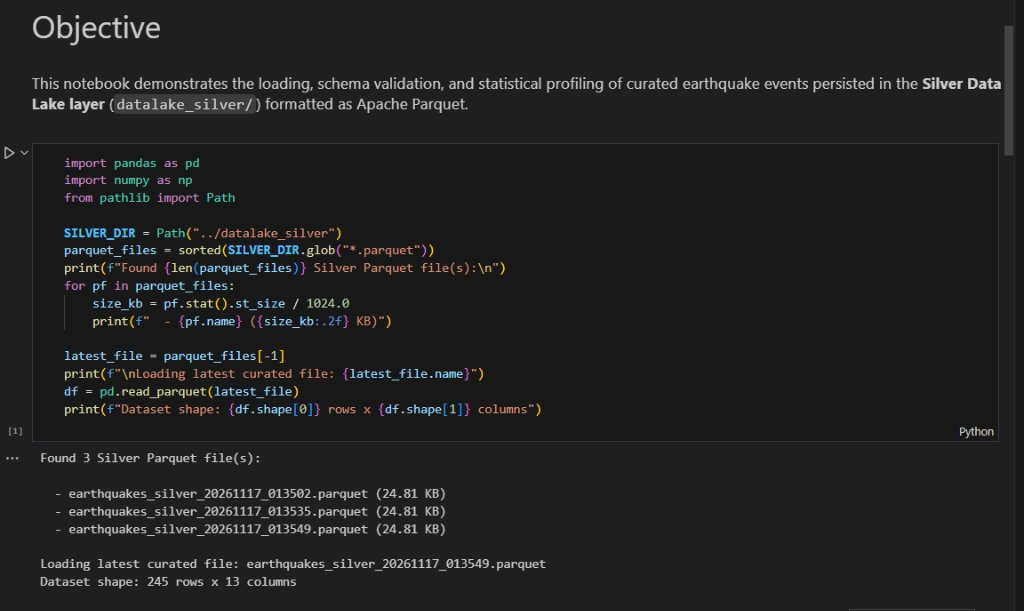
\includegraphics[width=0.95\columnwidth]{screenshots/06_notebook_parquet_loading.png}\\[0.2cm]
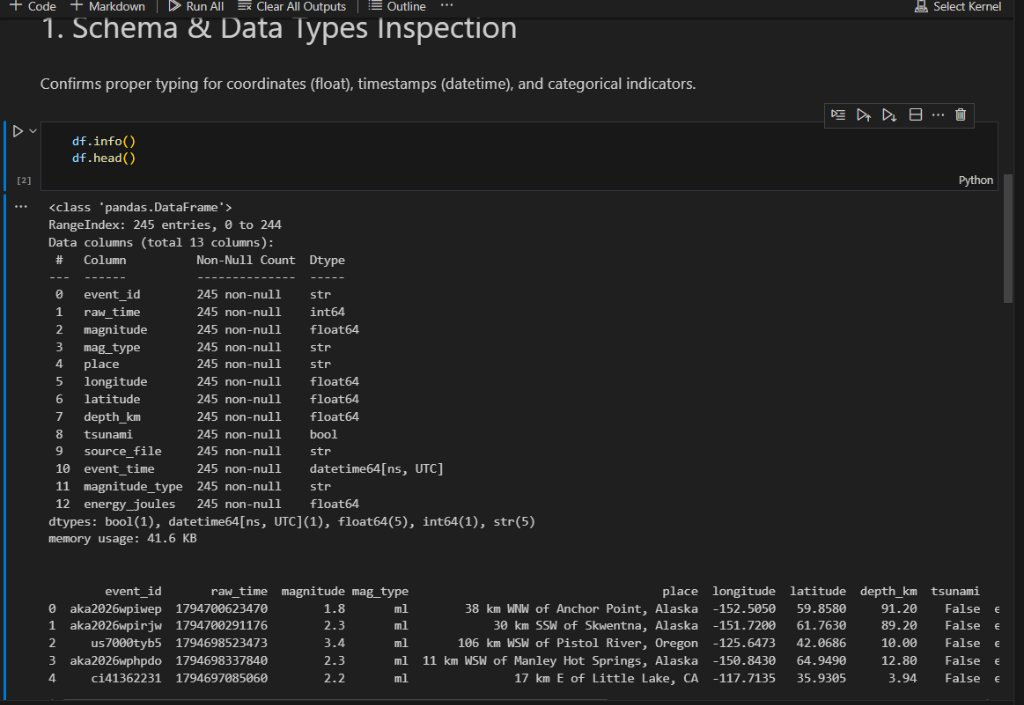
\includegraphics[width=0.95\columnwidth]{screenshots/07_notebook_schema_inspection.png}
\caption{Executed Jupyter Notebook (\texttt{02\_silver\_data\_exploration.ipynb}): Parquet file discovery, dataset shape ($245 \times 13$), and PyArrow schema verification.}
\label{fig:nb_1_2}
\end{figure}

\begin{figure}[!t]
\centering
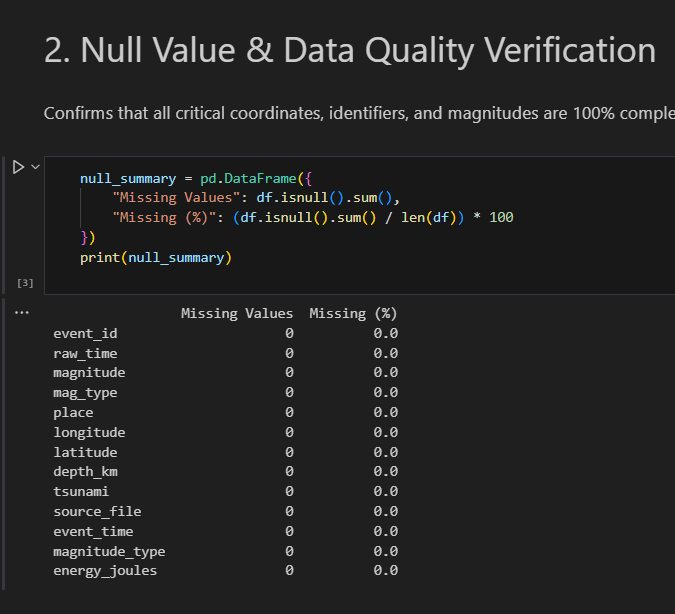
\includegraphics[width=0.92\columnwidth]{screenshots/08_notebook_null_verification.png}\\[0.18cm]
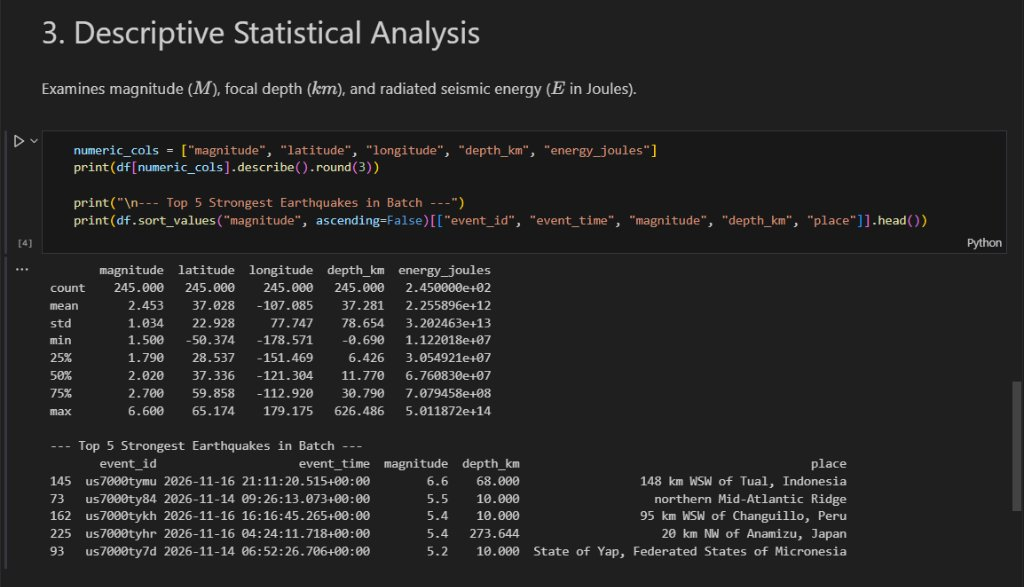
\includegraphics[width=0.95\columnwidth]{screenshots/09_notebook_descriptive_stats.png}\\[0.18cm]
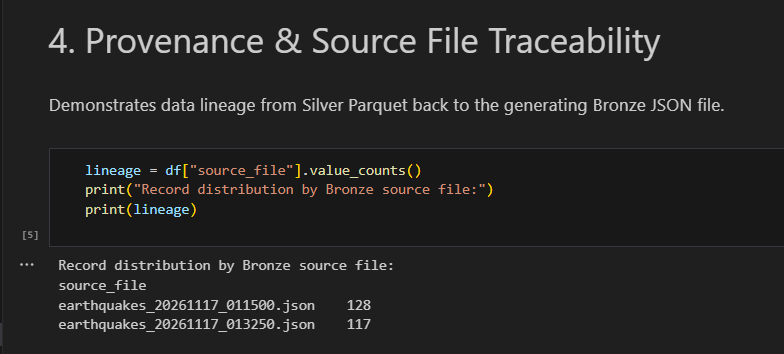
\includegraphics[width=0.92\columnwidth]{screenshots/10_notebook_provenance_lineage.png}
\caption{Executed Jupyter Notebook verification: (top) $0.0\%$ null rate across all 13 fields; (middle) descriptive statistics and top 5 strongest earthquakes; (bottom) Bronze-to-Silver file lineage distribution.}
\label{fig:nb_3_4_5}
\end{figure}
